\documentclass[a4paper,10pt]{article}
\usepackage[utf8]{inputenc}
\usepackage{graphicx}
\usepackage{amsmath}
\usepackage{amssymb}
\usepackage{amsthm}
\usepackage{booktabs}
\usepackage{caption}
\usepackage{geometry}
%\usepackage{hyperref}
\usepackage{makeidx}
\usepackage{microtype}
\usepackage{subfig}
\usepackage{tabularx}
\usepackage{url}
\usepackage{varioref}
\usepackage[italian]{babel}
\usepackage{xcolor}
\usepackage{multicol}
\usepackage{mathtools}
\usepackage{booktabs}
\usepackage{gensymb}


\title{Laboratorio I: Pendolo accoppiatio\\ Misura del periodo.\\
\begin{large}
Dipartimento di Fisica E.Fermi - Università di Pisa
\end{large}}

\author{Di Ubaldo Gabriele \\Giannelli Martina \\Torosantucci Andrea}
\date{2 Marzo 2016}

\begin{document}

\maketitle

\tableofcontents

%%%%%%%%%%%%%%%%%%%%%%%%%%%%%%%%%%%%%%%%%%%%%%%%%%%%%%%%%%%%%%%%%%%%%%%%%%%%%%%%%%%%%%%%%%%%%%%%%%%%%%%%%%%%%%%%%%%%%%%%%%%%%%%%%%%%%%%%%%%%%%%%%%%%%%%%%%%%%%%%%%%%%%%%%%%%%%%%%%%
\section{Introduzione}
\subsection{Teoria}
\textbf{Obiettivo:} Studiare il moto di due pendoli accoppiati attraverso una molla e il fenomeno ondulatorio dei battimenti.
In un sistema generico di due pendoli vi possono essere modi di oscillazione molto complessi ma con due particolari configurazioni iniziali possiamo ottenere un moto armonico scomponibile in 
modi normali. Queste configurazioni si chiamano di fase e di controfase. La frequenza di un solo pendolo è
\begin{equation}
 w_0=\sqrt{\frac{mgl}{I}}
\end{equation}
Se viene aggiunto uno smorazatore, nel nostro caso attraverso un gallegiante che risente di attrito viscoso, possiamo stimare il tempo di decadimento dell'ampiezza secondo la formula:
\begin{equation}
 A(t)=A_0 e^{-\frac{t}{\tau}}
\end{equation}
Il periodo rimane invariato nonostante vi sia attrito. 
In seguito andiamo a studiare il sistema di due pendoli e i due modi normali possibili sono ``in fase'' e ``in controfase''.
In un'oscillazione in fase nel sistema di riferimento di un pendolo l'altro è fermo poichè si muovono con la stessa frequenza, dunque la molla non è sollecitata e il periodo è uguale 
a quello di un pendolo singolo.
In un oscillazione in controfase i pendoli vengono spostati di ampiezze uguali in versi opposti. Si verifica allora che per $k$ piccoli della molla la frequenza del sistema sarà maggiore
di quello in fase ma di una quantità non significativa.
Se invece mettiamo in oscillazione solo uno dei due pendoli lasciando l'altro nella sua posizione di equilibrio si verifica il fenomeno dei battimenti in cui il moto è dato dalla somma 
dei modi normali. Nel caso specifico si hanno ampiezze uguali e differenza di fase massima. Quindi si ha
\begin{equation}
 x(t)=A_0[\cos(w_ft+\varphi_1)+\cos(w_ct+\varphi_2)]
\end{equation}
Usando le formule di prostaferesi
\begin{equation}
 \cos(\alpha)+\cos(\beta)=2*\cos(\frac{\alpha+\beta}{2})\cos(\frac{\alpha-\beta}{2})
\end{equation}
Da queste ricaviamo le frequenze portante e modulante:
\begin{equation}
 w_p=\frac{w_c+w_f}{2}\approx w_c, w_p
\end{equation}
\begin{equation}
 w_p=\frac{w_c-w_f}{2} \ll w_c, w_p
\end{equation}

\subsection{Apparato sperimentale}
\begin{itemize}
\item{Due pendoli di uguale massa e lunghezza}
\item{Supporto di sospensione}
\item{Molla di costante $k$}
\item{Programma di acquisizione dati Plasduino}
\item{Gallegiante da pesca}
\item{Metro a nastro con risoluzione di $1 mm$}
\end{itemize}

%%%%%%%%%%%%%%%%%%%%%%%%%%%%%%%%%%%%%%%%%%%%%%%%%%%%%%%%%%%%%%%%%%%%%%%%%%%%%%%%%%%%%%%%%%%%%%%%%%%%%%%%%%%%%%%%%%%%%%%%%%%%%%%%%%%%%%%%%%%%%%%%%%%%%%%%%%%%%%%%%%%%%%%%%%%%%%%%%%%
\section{Esperimento}
\subsection{Acquisizione misure}
Per primo abbiamo misurato con Plasduino il periodo del pendolo singolo non smorzato: $T=1.40\pm0.001s$. Il periodo teorico è $T=1.40s0$
\\In secondo luogo abbiamo misurato con Plasduino il periodo del pendolo singolo smorazto: $T=1.40s\pm0.001s$. Inoltre abbiamo determinato il tempo caratteristico $\tau\approx40s$.
Il tempo caratteristico l'abbiamo trovato dividendo per $e$ l'ampiezza all'inizio dell'osccillazione e trovando un punto nel tempo la cui ampiezza fosse $A_0/e$.
\\In terzo luogo abbiamo misurato con Plasduino il periodo del pendolo accoppiato in fase: $T=1.40s\pm0.001s$.
\\In quarto luogo abbiamo misurato con Plasduino il periodo del pendolo accoppiato in controfase $T=1.37s\pm0.01s$

\subsection{Analisi Dati}
L'errore sul periodo teorico del pendolo singolo è:

Dai periodi dei pendoli accoppiati possiamo calcolare le frequenze portante e modulante:
$w_p=(4.48+4.58)/2=4,53 rad/s$
$w_m=0.05 rad/s$
Abbiamo usato i dati del sistema in controfase e i dati dei battimenti per fare un fit curvilineo usando un programma in Python. Con il programma può essere fatto il fit anche delle 
altre configurazioni.

\begin{figure}[!htb]
\begin{center}
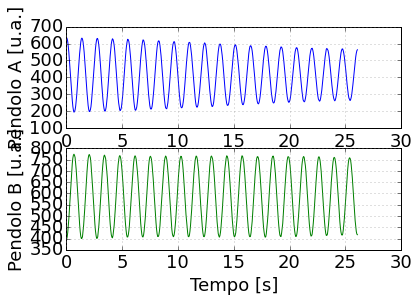
\includegraphics[width=10cm]{dati/controfase.png}
\end{center}
\end{figure}

\begin{figure}[!htb]
\begin{center}
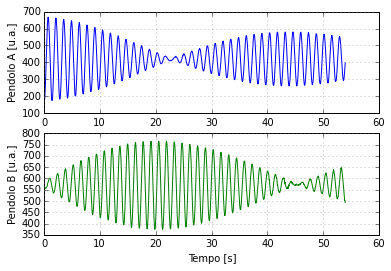
\includegraphics[width=10cm]{dati/battimenti.png}
\end{center}
\end{figure}



\section{Conclusione}
La teoria è in accordo con i dati raccolti: il periodo del pendolo è uguale sia se libero che se smorzato, il periodo in fase è uguale al periodo singolo e il periodo in controfase è 
leggermente minore di questo
\end{document}


